\documentclass[fontsize=12pt,a4paper]{scrartcl}
 
% Das Prozent-Zeichen leitet einen Kommentar ein,
% es hilft ebenso, im Text Leerzeichen zu unterbinden.
 
% fontsize=12pt  Schriftgroesse in 10, 11 oder 12 Punkt
% a4paper        Papierformat ist hier A4
% landscape      Querformat wird natürlich unterstützt ;-)
% parskip        Absatzabstand anstatt Einzüge
% draft          Der Entwurfsmodus deckt Schwächen auf
% {scrartcl}     Die Dokumentenklasse book, report, article
%                oder fürs deutsche scrbook, scrreprt, scrartcl
 
%\usepackage[ngerman]{babel} % Deutsche Sprachanpassungen
\usepackage[T1]{fontenc}    % Silbentrennung bei Sonderzeichen
\usepackage[latin1]{inputenc} % Direkte Angabe von Umlauten im Dokument.
                            % Wenn Sie an einem Mac sitzen,verwenden
                            % Sie ggf. „macce“ anstatt „utf8“.
 
\usepackage{textcomp}       % Zusätzliche Symbolzeichen
\usepackage{siunitx}
\usepackage{amsmath}
\usepackage{listings}
\usepackage{graphicx}
\lstset{tabsize=4, showspaces=false}


\title{Machine Learning SS2013}
\subtitle{Ulrike von Luxburg \\ Assignment 02}
\author{Arne Schr�der \and Falk Oswald \and Angel Bakardzhiev}
 
\date{\today}               % \today setzt das heutige Datum
 
\begin{document}
\maketitle                  % Titelei erzeugen
% \tableofcontents            % Inhaltsverzeichnis anlegen
 
 
\section*{Matlab Implementation}
First, we introduce and briefly describe our M files, included in the attached zip file.

\begin{itemize}
	\item \textbf{knnClassify.m} - function, that uses k-nearest neighbours method to predict labels
	\item \textbf{evaluateK.m} - evaluates knnClassify for different k-values and returns the minimal k
	\item \textbf{loss01.m} - Gets as input a prediction calculated by the knnClasifiy and correct labels y. The function returns the average error (empirical risk with respect to the 0-1 loss) for this prediction.
	\item \textbf{doExercise1.m} - loads all training and test data for exercise 1, calls knnClassify and plots the result
	\item \textbf{doExercise2.m} - loads all training and test data for exercise 2, calculates and plots the results
	\item \textbf{Assignment02.m} - the main script, calls doExercise1 and doExercise2 with different parameters, also contains the code for exercise 4
\end{itemize}
 
\section*{Exercise 5}

\subsection*{Question 1}

What are false positive, false negative and average error of you(r) calssifier?

\subsection*{Answer}

To answer this question we simply need to fill out the following table:\\

\begin{tabular}{c||c|c|c}
& spam & not spam & overall \\ 
\hline\hline
 classified as spam &  &  &  \\ 
\hline
 classified as not spam &  &  &  \\ 
\hline
 overall & 60 \% &  & 
\end{tabular} 

We know that 85 \% of spam is classified as such, which gives us that $60 \% \cdot 85 \% = 51 \%$ of mails are spam and are classified as spam.

As 60 \% of all mail is spam, 40 \% of mail is not. This means that if 5 \% of all non-spam mails are classified as spam this is 2 \% of all mails.\\

\begin{tabular}{c||c|c|c}
& spam & not spam & overall \\ 
\hline\hline
 classified as spam & 51 \% & 2 \% &  \\ 
\hline
 classified as not spam &  &  &  \\ 
\hline
 overall & 60 \% & 40 \% & 
\end{tabular}

Subtraction now tells us that 9 \% of mails are spam but not classified spam and 38 \% are spam and correctly classified.\\

\begin{tabular}{c||c|c||c}
& spam & not spam & overall \\ 
\hline\hline
 classified as spam & 51 \% & 2 \% & 53 \% \\ 
\hline
 classified as not spam & 9 \% & 38 \% & 47 \% \\ 
\hline \hline
 overall & 60 \% & 40 \% & 100 \%
\end{tabular}

Therefore, the false positive rate is 2 \% and the false negative rate is 9 \%.

\section*{Task 2}

Find a classification algorithm with false positive rate 0. Find a classification algorithm with false negative rate 0.

\section*{Solution}

An algorithm with false positive rate of 0 can be achieved by not classifying anything as spam (resulting in a 40 \% false negative rate).

Conversely, an algorithm with false negative rate of 0 can be achieved by classifying everything as spam (resulting in a 60 \% false positive rate).

\section*{Question 3}

Which entries of $X'$ lead to a false positive error and which ones to a false negative error in the Bayes classification?

\section*{Answer}

The false positives are those classified as 2 but being 1, in this case this applies to 2.5. The false negatives are those classified as 1 but being 2, in this case this applies to 2.

\section*{Task 4}

Sketch the approximate Bayesian decision boundary by hand with respect to the following loss functions
\begin{itemize}
\item[-] 0-1 loss
\item[-] Unsymmetric los(s): $\ell(\text{spam},\text{non-spam}) = 1$, $\ell(\text{non-spam},\text{spam}) = 100$.
\end{itemize}

\section*{Solution}

The first is the same as if there was no loss function. In the following graph, one can see a with solid lines the decision curves for none or a 0-1 loss function and with dashed lines are the decision curves for the asymmetric loss. Magenta being in favour for 1 (non-spam) and black being in favour for 2 (spam):
\begin{center}
  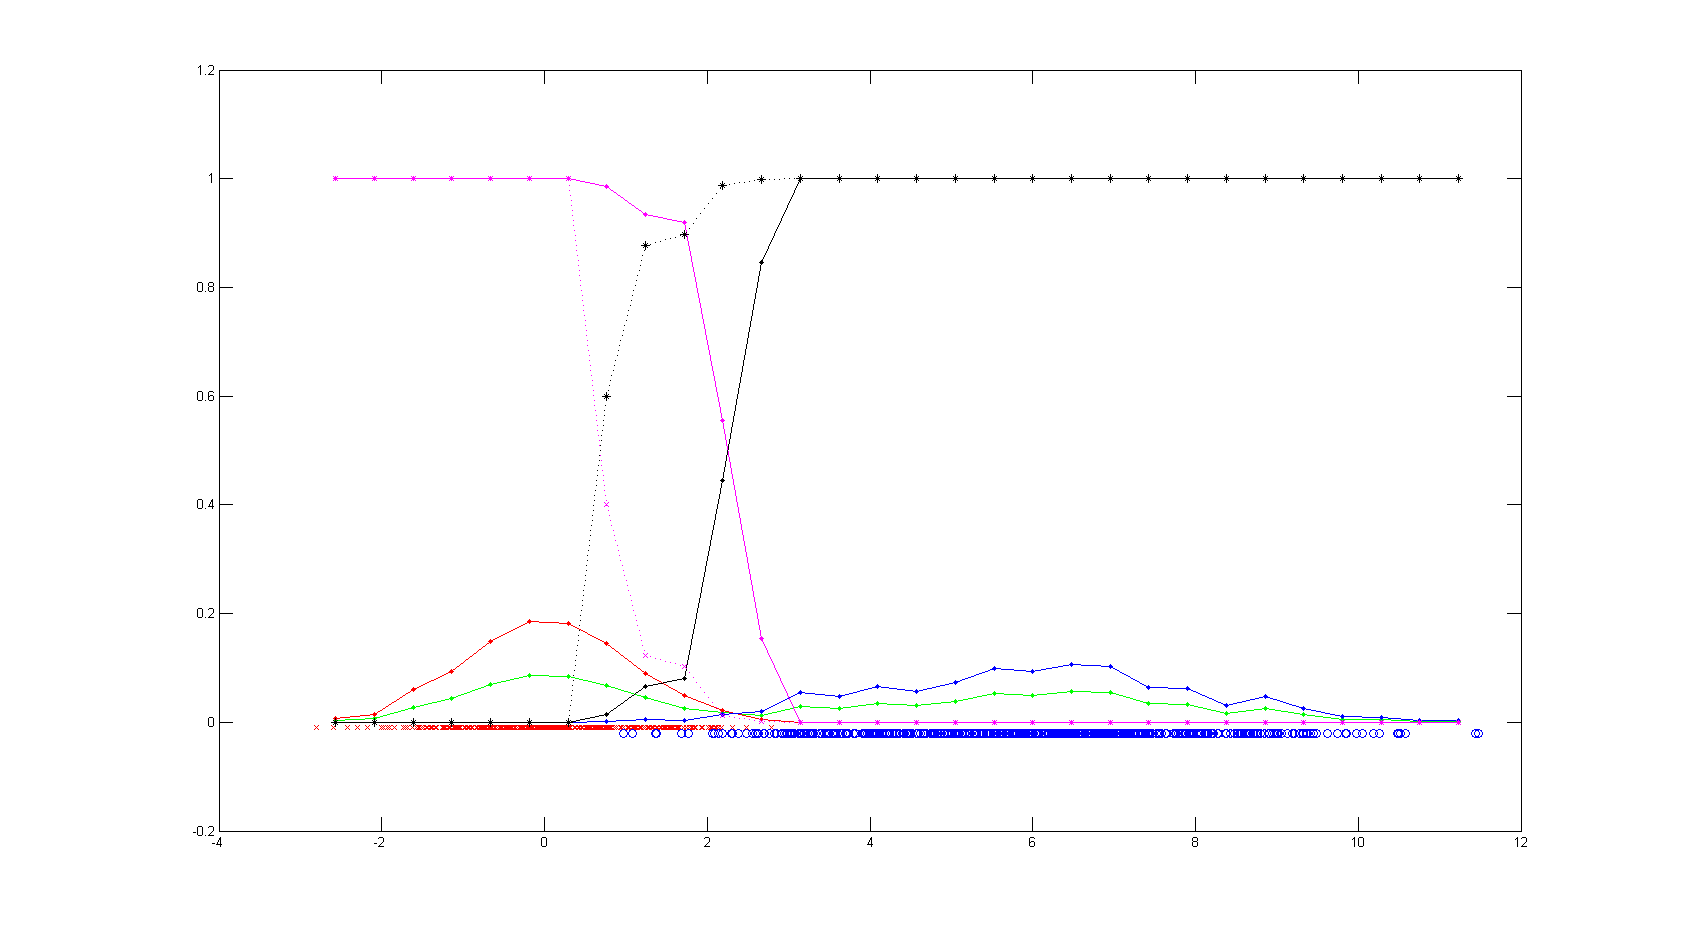
\includegraphics[width=\textwidth]{decision_graph.png}
\end{center}

\end{document}